\chapter{}

\section{Screenshots}
\justify

The following screenshots illustrate the model training process and evaluation outputs from Experiment 7 (RF-DETR Medium, 1024$\times$1024 patches, 35\% overlap).

\begin{figure}[H]
\centering
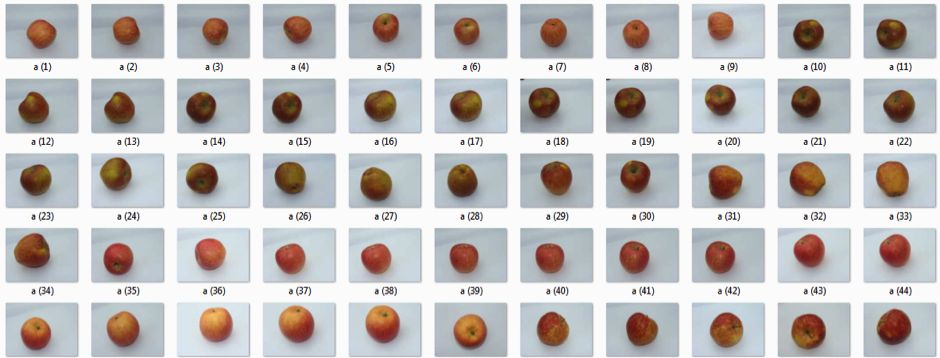
\includegraphics[width=0.8\textwidth]{images/ScreenShots/Training.png}
\caption{RF-DETR Medium training progress (Experiment 7). Loss curves and mAP metrics tracked across 20 epochs.}
\end{figure}

\begin{figure}[H]
\centering
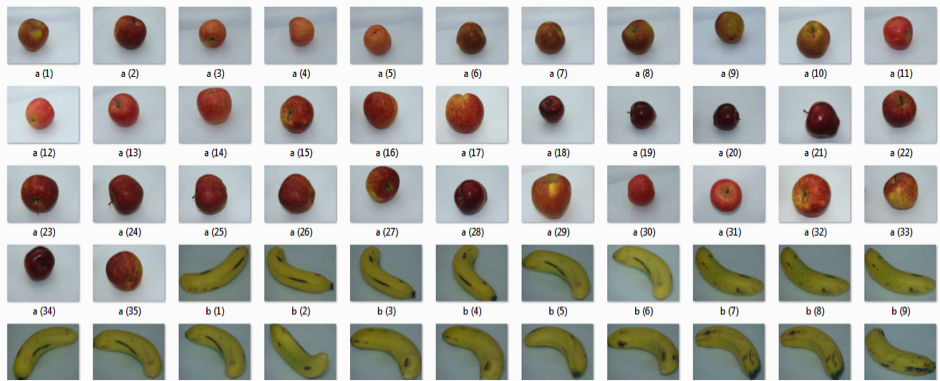
\includegraphics[width=0.8\textwidth]{images/ScreenShots/TestSet.png}
\caption{Sample inference results on the test split. Bounding boxes shown for detected Crack (red) and Cold Shut (blue) defects.}
\end{figure}

\begin{figure}[H]
\centering
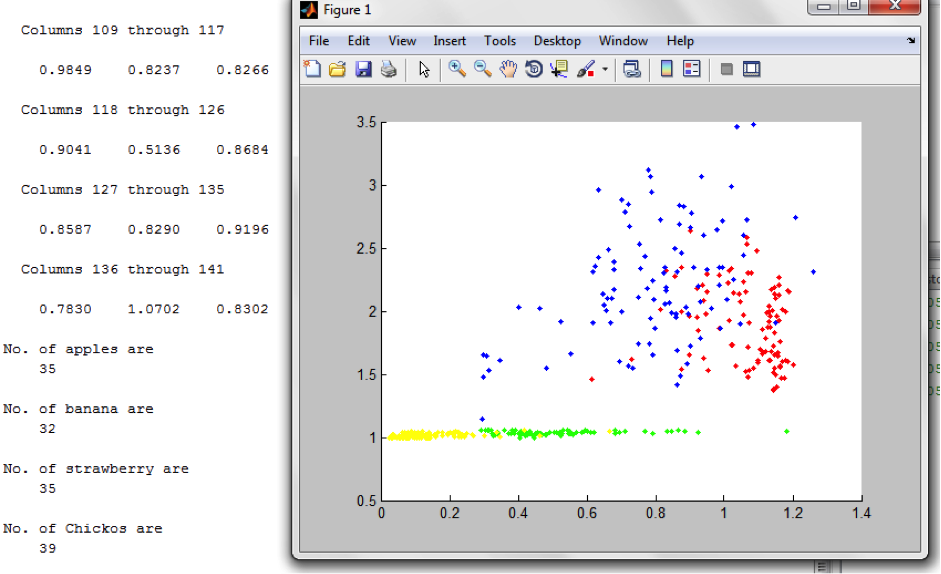
\includegraphics[width=0.8\textwidth]{images/ScreenShots/DistClass.png}
\caption{Class distribution in the patch dataset after augmentation. Crack and Cold Shut annotation counts shown for the training split.}
\end{figure}

\section{Gantt Chart}
\justify

The project was executed across two semesters following a structured experimental plan. Key milestones included: dataset acquisition and EDA (Weeks 1--3), patch pipeline development (Weeks 4--6), baseline training Experiment 1 (Week 7), dataset engineering Experiments 2--6 (Weeks 8--12), final training Experiment 7 (Weeks 13--14), report writing and review (Weeks 15--16).

\section{Glossary}
\justify

\begin{description}[leftmargin=3cm, style=nextline]
    \item[HPDC] High-Pressure Die Casting --- a manufacturing process where molten metal is injected into reusable dies at high pressure.
    \item[RF-DETR] Roboflow Detection Transformer --- an Apache 2.0 end-to-end object detection model based on DINOv2 and deformable DETR.
    \item[mAP50-95] Mean Average Precision averaged over IoU thresholds from 0.50 to 0.95 in steps of 0.05 (COCO standard metric).
    \item[EMA] Exponential Moving Average --- a smoothing technique applied to model weights during training to improve generalisation.
    \item[COCO] Common Objects in Context --- a standard annotation format and evaluation benchmark for object detection.
    \item[Patch] A fixed-size cropped sub-region of a full image, used as an individual training sample in the sliding-window strategy.
    \item[NMS] Non-Maximum Suppression --- a post-processing step to remove duplicate detections (not required by RF-DETR).
    \item[GIoU] Generalised Intersection over Union --- a bounding box regression loss function.
    \item[ViT] Vision Transformer --- a transformer-based image backbone that processes images as sequences of patches.
    \item[DINOv2] A self-supervised ViT pre-training method from Meta AI providing strong visual representations.
    \item[AP] Average Precision --- area under the precision-recall curve for a single class at a given IoU threshold.
\end{description}

\section{Description of Tools and Technology Used}
\justify

\begin{table}[H]
\centering
\caption{Tools and Technologies}
\begin{tabular}{lll}
\toprule
\rowcolor{tableHeader}\tableheadfont Tool / Library & \tableheadfont Version & \tableheadfont Purpose \\
\midrule
Python           & 3.10     & Primary programming language \\
\rowcolor{tableRowAlt}PyTorch          & 2.0+     & Deep learning framework \\
RF-DETR          & Roboflow 2025 & Object detection model \\
\rowcolor{tableRowAlt}Shapely          & 2.0      & Polygon clipping for patch generation \\
OpenCV           & 4.8      & Image loading and annotation rendering \\
\rowcolor{tableRowAlt}pycocotools      & 2.0      & COCO-standard mAP evaluation \\
NumPy            & 1.24     & Array operations \\
\rowcolor{tableRowAlt}Matplotlib       & 3.7      & Visualisation and training curves \\
NVIDIA RTX 6000 Ada & 49 GB VRAM & GPU for model training \\
\rowcolor{tableRowAlt}CUDA             & 11.8     & GPU compute platform \\
Ubuntu           & 22.04 LTS & Operating system \\
\bottomrule
\end{tabular}
\end{table}

\section{Blueprint}

The system architecture blueprint and data flow diagram are provided in Figure~\ref{fig:rfdetr_arch} (Chapter 4) and Figure~\ref{fig:system_overview} (Chapter 3).

\section{Plagiarism Report}

Attach the Turnitin / iThenticate plagiarism report at the end of this appendix.
